\documentclass[a4paper, 10pt, twocolumn]{article}
\usepackage{amssymb}
\usepackage{cellspace, graphicx, makecell}
\usepackage{graphicx} % Required for inserting images
\usepackage[utf8]{inputenc}
\usepackage[T2A]{fontenc}
\usepackage[english,russian]{babel}
\usepackage{cmap}
\usepackage[left=1cm,right=1cm,
    top=1cm,bottom=2cm]{geometry}
\usepackage{paracol}
\usepackage{multicol}
\usepackage{amsmath}
\usepackage{lipsum}
\usepackage{vwcol}
\usepackage{float}

% Установка размера формул
\DeclareMathSizes{10}{10}{10}{10}   % Для основного текста размером 10pt

\title{Лабораторная работа 2.1.1 \\ Измерение удельной теплоёмкости воздуха при постоянном
давленини}
\author{Матвей Галицын \\ Б01-411}
\date{February 5, 2024}

\setlength{\columnseprule}{0.1pt}
\setlength{\columnsep}{3em}
\raggedbottom
\begin{document}
\maketitle
\newpage{}
\section{Аннотация}
    \subsection{Задача}
        В работе определяется коэффициент теплопроводности воздуха при атмосферном давлении и разных 
        температурах по теплоотдаче нагреваемой током нити в цилиндрическом сосуде.
    \subsection{Оборудование}
        Прибор для определения теплопроводности газов, форвакуумный насос, термостат, магазин 
        сопротивлений, цифровой вольтметр В7-38, эталонное сопротивление 10 Ом, источник питания.
\section{Теория}
    Основной характеристикой теплопроводности служит коэффициент $\varkappa$, являющийся коэффициентом 
    пропорциональности между плотностью потока тепла $q$ и градиентом температуры $dT/dr$ в направлении
     распространения этого потока $$ q = -\varkappa \frac{dT}{dr} \eqno{(1)}$$

	В цилиндрически симметричной установке, в которой тепловой поток направлен к стенкам цилиндра от
     нити, полынй поток тепла $Q = qS$ через каждую цилиндрическую поверхность радиуса $r$ должен в 
     стационарном состоянии быть неизменен (как в пространстве, так и во времени). Тогда:
    $$Q = -2\pi rL\varkappa \frac{dT}{dr} = const, \eqno{(2)}$$
    откуда получаем формулу $$ T_1 - T_2 = \frac{Q}{2\pi L\varkappa} \ln \frac{r_2}{r_1} \eqno{(3)}$$
                            $$ \varkappa = \frac{Q}{2\pi L (T_1 - T_2)} \ln \frac{r_2}{r_1} \eqno{(\widehat{3})}$$
    Здесь $r_1$ и $T_1$ -- радиус и температура нити, $r_2$ и $T_2$ -- радиус и температура цилиндра.
\section{Экспериментальная установка}
    \begin{figure}[H]
        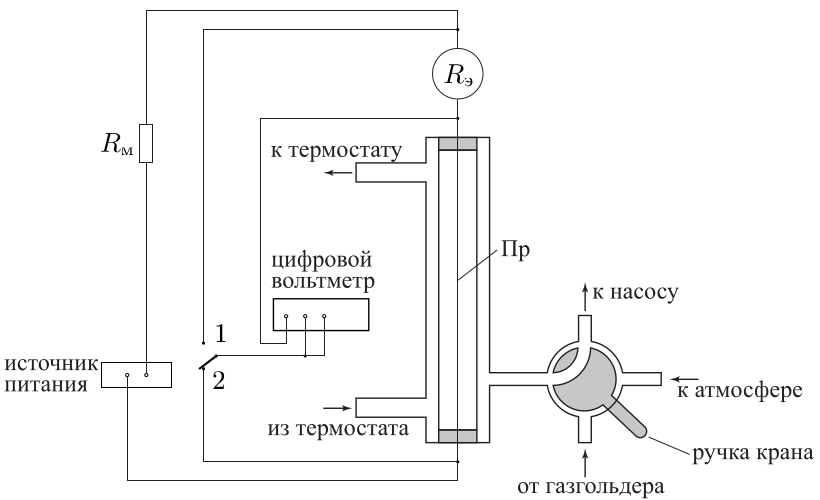
\includegraphics[width=1\linewidth]{images/installation.png}
        \begin{center}
            \caption{Экспериментальная установка}
        \end{center}
    \end{figure}
    Схема установки изображена на рис. 1. Тонкая нить (никелевая или 
    вольфрамовая проволока) натянута по оси длинной вертикально стоящей медной трубки1. Через штуцер
     трубка заполняется исследуемым газом. Нить нагревается электриче- ским током, её температура Т1
     определяется по изменению электриче- ского сопротивления. Трубка находится в кожухе, через 
    который пропускается вода из термостата. Температура воды Т2 измеряется термо- метром, помещённым
     в термостат. Количество теплоты, протекающей через газ, равно (если пренебречь утечками тепла 
     через торцы) коли- честву теплоты, выделяемому током в нити, и может быть найдено по закону 
    Джоуля-Ленца. При этом ток в нити определяется по напряже- нию на включённом последовательно с 
    ней эталонном сопротивлении 10 Ом. Таким образом, все величины, входящие в правую часть формулы 
    $(\widehat{3})$, поддаются непосредственному измерению.
    \\ \newline
    Электрическая часть схемы состоит из источника питания и подклю- чённых к нему последовательно 
    соединённых нити, эталонного сопро- тивления 10 Ом и магазина сопротивлений RM, служащего для 
    точной установки тока через нить. Цифровой вольтметр может подключаться как к нити, так и к 
    эталонному сопротивлению, измеряя таким образом напряжение на нити и ток через неё.
    \\ \newline
    При определённой температуре термостата снимается зависимость напряжения на нити от тока, 
    проходящего через неё. Затем по полу- ченным данным строится график зависимости рассеиваемой 
    мощности от сопротивления нити, по которому можно определить сопротивление нити при нулевом токе,
     то есть при температуре термостата. Это сопро- тивление затруднительно измерить непосредственно
     из-за термоэлек- трических явлений, заметно искажающих результаты при малых токах, большие же 
    токи существенно изменяют температуру нити. Повторив эти измерения при различных температурах 
    термостата, можно опре- делить температурную зависимость сопротивления нити. Коэффициент 
    теплопроводности определяется затем по зависимости выделяемой мощ ности от разности температур с
     помощью формулы $(\widehat{3})$. При небольших значениях разности температур эта зависимость хорошо 
    аппроксимируется прямой.
\section{Результаты измерений и обработка данных}
    Далее приведены результаты экспериментов при T = 23.4 °C, 33.4 °C, 48.4 °C, 58.4 °C и 68.4 °C.
    Сразу за каждой таблицей идет график зависимости $R_\text{н}(Q)$, где $R_\text{н}$ - сопротивление нити, 
    Q - выделяемая  мощность. \newline
    Угловой коэффициент касательной можно расчитывать по методу наименьших квадратов.
    $$k = \frac{\left\langle R \cdot Q \right\rangle - \left\langle R \right\rangle \left\langle Q \right\rangle}
    {\left\langle Q^2 \right\rangle - \left\langle Q \right\rangle^2}$$
    Смещение по вертикали: $$R_0 = \left\langle R \right\rangle - k \cdot \left\langle Q \right\rangle^2$$
    \subsection{T = 23.4 °C}
    График для первого случая приведен в приложении.
    \begin{figure}[H]
        \centering
        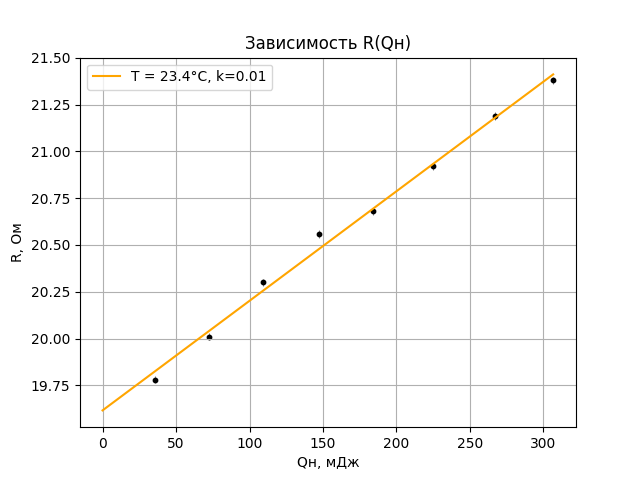
\includegraphics[width=1\linewidth]{graphs/figure1.png}
        \begin{center}
            \caption{График зависимости при $T =23.4 \, ^\circ\text{C}$ $R_\text{н}(Q)$}
        \end{center}
    \end{figure}


    \subsection{T = 33.4 °C}
    \begin{table}[H]
        \centering
        \begin{tabular}{|c|c|c|c|c|} \hline
        № & $U$, В & $I, \text{мА}$ & $ Q, \text{мВт} $ & $R_\text{н}, \text{Ом}$ \\ \hline
        1 & 0.84 & 41.33  & 34.56  & 20.42 \\ \hline
        2 & 1.20 & 58.12  & 69.74  & 20.65 \\ \hline
        3 & 1.50 & 71.10  & 107.40 & 20.95 \\ \hline
        4 & 1.75 & 82.67  & 144.69 & 21.17 \\ \hline
        5 & 1.99 & 92.90  & 184.87 & 21.42 \\ \hline
        6 & 2.18 & 101.17 & 220.55 & 21.55 \\ \hline
        7 & 2.38 & 109.36 & 260.30 & 21.76 \\ \hline
        8 & 2.57 & 116.88 & 300.38 & 21.98 \\ \hline
        \end{tabular}
        \caption{$R_\text{н}(Q)$ при T = 23.4 °C}
    \end{table}
    \begin{figure}[H]
        \centering
        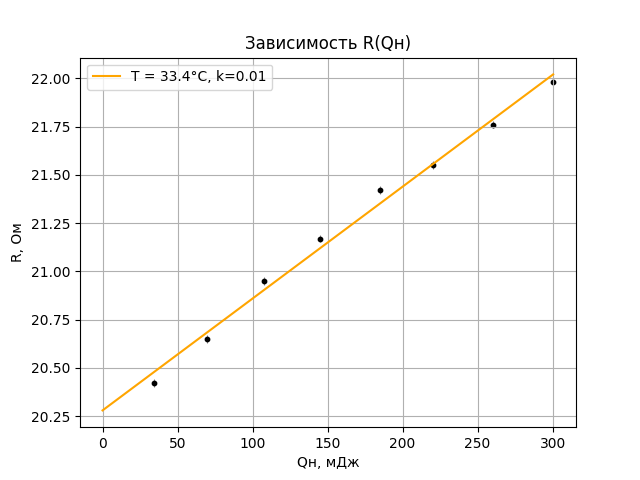
\includegraphics[width=1\linewidth]{graphs/figure2.png}
        \begin{center}
            \caption{График зависимости при $T =33.4 \, ^\circ\text{C}$ $R_\text{н}(Q)$}
        \end{center}
    \end{figure}
    В данном случае $R_0 = 20.27$

    \subsection{T = 48.4 °C}
    \begin{table}[H]
        \centering
        \begin{tabular}{|c|c|c|c|c|} \hline
        № & $U$, В & $I, \text{мА}$ & $ Q, \text{мВт} $ & $R_\text{н}, \text{Ом}$ \\ \hline
        1 & 0.86 & 40.06  & 34.45  & 21.47 \\ \hline
        2 & 1.23 & 56.43  & 69.41  & 21.80 \\ \hline
        3 & 1.52 & 69.07  & 104.99 & 22.01 \\ \hline
        4 & 1.80 & 80.91  & 145.64 & 22.25 \\ \hline
        5 & 2.00 & 89.52  & 179.04 & 22.34 \\ \hline
        6 & 2.21 & 97.78  & 216.09 & 22.06 \\ \hline
        7 & 2.40 & 105.52 & 253.25 & 22.75 \\ \hline
        8 & 2.59 & 112.5  & 292.31 & 22.95 \\ \hline
        \end{tabular}
        \caption{$R_\text{н}(Q)$ при T = 48.4 °C}
    \end{table}

    \begin{figure}[H]
        \centering
        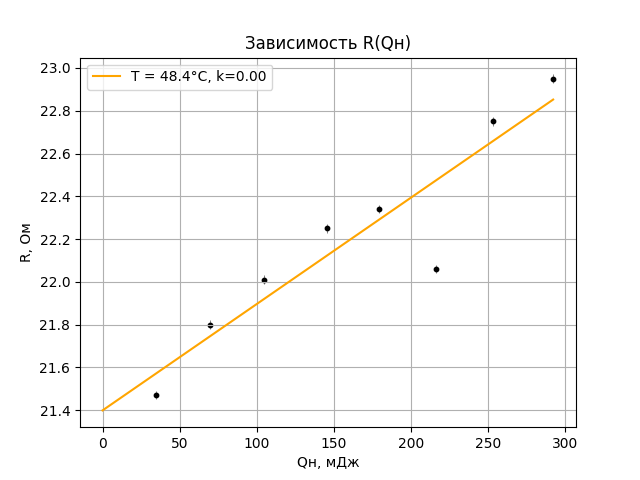
\includegraphics[width=1\linewidth]{graphs/figure3.png}
        \begin{center}
            \caption{График зависимости при $T =48.4 \, ^\circ\text{C}$ $R_\text{н}(Q)$}
        \end{center}
    \end{figure}
    В данном случае $R_0 = 21.4$

    \subsection{T = 58.4 °C}
    \begin{table}[H]
        \centering
        \begin{tabular}{|c|c|c|c|c|} \hline
        № & $U$, В & $I, \text{мА}$ & $ Q, \text{мВт} $ & $R_\text{н}, \text{Ом}$ \\ \hline
        1 & 0.87 & 39.24  & 34.14  & 22.17 \\ \hline
        2 & 1.25 & 55.36  & 69.20  & 22.58 \\ \hline
        3 & 1.54 & 67.64  & 104.17 & 22.76 \\ \hline
        4 & 1.79 & 78.05  & 139.71 & 22.93 \\ \hline
        5 & 2.01 & 87.42  & 175.71 & 22.99 \\ \hline
        6 & 2.22 & 95.56  & 212.14 & 23.23 \\ \hline
        7 & 2.42 & 103.29 & 249.96 & 23.43 \\ \hline
        8 & 2.61 & 110.44 & 288.15 & 23.63 \\ \hline
        \end{tabular}
        \caption{$R_\text{н}(Q)$ при T = 58.4 °C}
    \end{table}

    В данном случае $R_0 = 21.4$

    \begin{figure}[H]
        \centering
        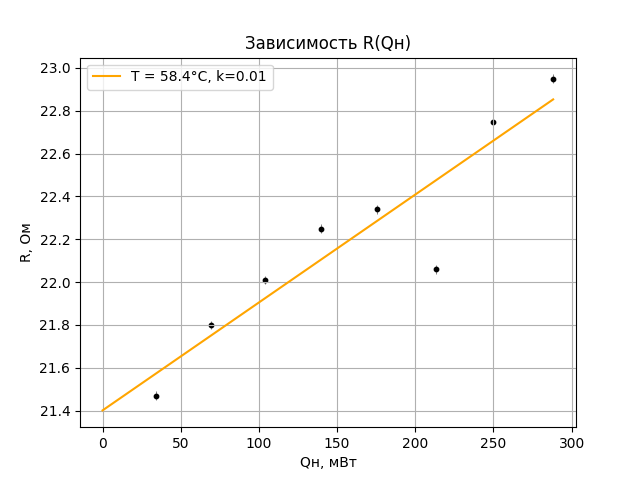
\includegraphics[width=1\linewidth]{graphs/figure4.png}
        \begin{center}
            \caption{График зависимости при $T =58.4 \, ^\circ\text{C}$ $R_\text{н}(Q)$}
        \end{center}
    \end{figure}

    \subsection{T = 68.4 °C}
    \begin{table}[H]
        \centering
        \begin{tabular}{|c|c|c|c|c|} \hline
        № & $U$, В & $I, \text{мА}$ & $ Q, \text{мВт} $ & $R_\text{н}, \text{Ом}$ \\ \hline
        1 & 0.88 & 38.17  & 33.59  & 23.05 \\ \hline
        2 & 1.25 & 54.08  & 67.60  & 23.11 \\ \hline
        3 & 1.55 & 66.14  & 102.57 & 23.44 \\ \hline
        4 & 1.80 & 76.59  & 137.86 & 23.50 \\ \hline
        5 & 2.03 & 85.40  & 173.36 & 23.77 \\ \hline
        6 & 2.24 & 93.41  & 208.24 & 23.98 \\ \hline
        7 & 2.44 & 101.17 & 246.85 & 24.12 \\ \hline
        8 & 2.62 & 108.03 & 289.04 & 24.25 \\ \hline
        \end{tabular}
        \caption{$R_\text{н}(Q)$ при T = 68.4 °C}
    \end{table}
    \begin{figure}[H]
        \centering
        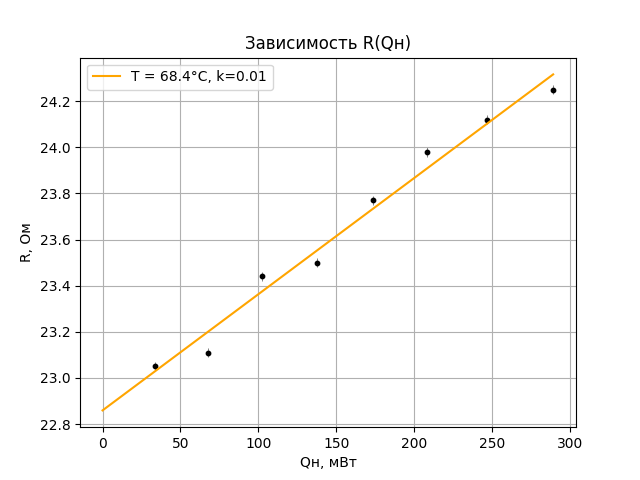
\includegraphics[width=1\linewidth]{graphs/figure5.png}
        \begin{center}
            \caption{График зависимости при $T =68.4 \, ^\circ\text{C}$ $R_\text{н}(Q)$}
        \end{center}
    \end{figure}

    В данном случае $R_0 = 22.85$
    \subsection{График зависимости $R$ от T}
    График в данном случае строим также по методу наименьших квадратов.
    \begin{table}[H]
        \centering
        \begin{tabular}{|c|c|c|} \hline
        № & $R, \text{Ом}$ & $T, ^\circ\text{C} $ \\ \hline
        1 & 18.6  & 23.4 \\ \hline
        2 & 20.27 & 33.4 \\ \hline
        3 & 21.4  & 48.4 \\ \hline
        4 & 21.4  & 58.4 \\ \hline
        5 & 22.85 & 68.4 \\ \hline
        \end{tabular}
        \caption{$R_\text{н}(Q)$ при T = 68.4 °C}
    \end{table}
    \begin{figure}[H]
        \centering
        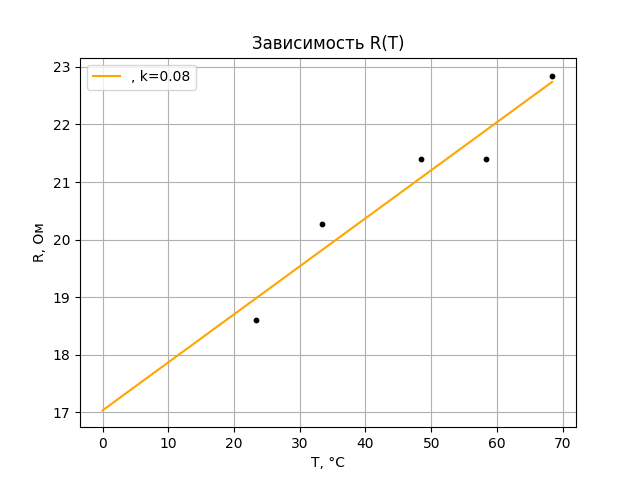
\includegraphics[width=1\linewidth]{graphs/figure6.png}
        \begin{center}
            \caption{Зависимость сопротивления от температуры}
        \end{center}
    \end{figure}
    С помощью угла наклона найдем коэффициент сопротивления: $$\alpha = \frac{1}{R_{273}}\frac{dR_0}{dt} \approx 0.005 \frac{1}{\text{°C}} $$

    Погрешность $\sigma_\alpha = \frac{1}{\sqrt{n}}\cdot \sqrt{\frac{\langle R^2 \rangle - \langle R \rangle ^2}{\langle T^2 \rangle - \langle T \rangle ^2} - R_0^2} = 
    \frac{1}{\sqrt{5}}\cdot\sqrt{\frac{438.98 - 436.97}{2418.96 - 2152.97} - 0.083^2} \approx 0.0001 \frac{1}{\text{°C}}$
    \subsection{Зависимость выделяющейся на нити мощности от её перегрева}

    Используя данные из предыдущих пунктов найдём зависимость выделяющейся на нити мощности $Q$ от её
     перегрева $\Delta T$ относительно стенок. Используя формулу $(\widehat{3})$ найдём коэффициенты
      теплопроводности воздуха.
    $$\frac{dQ}{d(\Delta T)} = \frac{dR_0}{dT} / \frac{dR}{dQ}$$

    $$k = \frac{dQ}{d(\Delta T)} / \frac{2 \pi L}{ln \frac{r_0}{r_1}} = \frac{dR_0}{dT} \frac{ln \frac{r_0}{r_1}}{2 \pi L} / \frac{dR}{dQ}$$

    $$\epsilon = \sqrt{ \left( \frac{\sigma_L}{L} \right)^2  + \left( \frac{\sigma_T}{T} \right)^2 + 
    \left( \frac{\sigma_\alpha}{\alpha}\right)^2} = \sqrt{\left( \frac{0.2}{40} \right)^2 + \left( \frac{0.2}{T} \right)^2}$$
    \begin{table}[H]
        \centering
        \begin{tabular}{|c|c|c|c|c|} \hline
        № & $T, ^\circ\text{C} $ & $\varkappa, 10^{-3}\frac{\text{Вт}}{\text{м} \cdot \text{c}}$ & $ \epsilon_\varkappa $ & $ \sigma_\varkappa, 10^{-3}\frac{\text{Вт}}{\text{м} \cdot \text{c}} $\\ \hline
        1 & 23.4 & 29.71 & 0.010 & 0.3 \\ \hline
        2 & 33.4 & 30.01 & 0.009 & 0.3 \\ \hline
        3 & 48.4 & 35.02 & 0.008 & 0.3 \\ \hline
        4 & 58.4 & 34.54 & 0.006 & 0.2 \\ \hline
        5 & 68.4 & 32.30 & 0.006 & 0.2 \\ \hline
        \shortstack{Среднее \\ значение} & & 32.3 & & 0.3 \\ \hline
        \end{tabular}
        \caption{$R_\text{н}(Q)$ при T = 68.4 °C}
    \end{table}
    \subsection{Зависимость теплопроводности воздуха от температуры}
    Строим зависимость $ln(\varkappa)$ от $ln(T)$ и находим коэффициент наклона $\beta$.

    \begin{figure}[H]
        \centering
        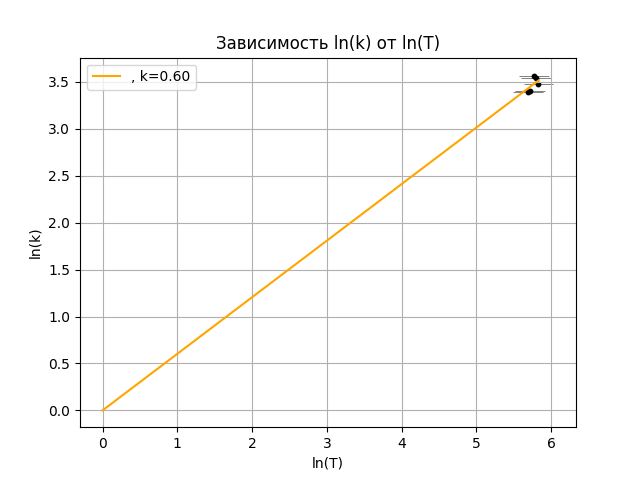
\includegraphics[width=1\linewidth]{graphs/figure7.png}
        \begin{center}
            \caption{Зависимость ln(k) от ln(T)}
        \end{center}
    \end{figure}

    Таким образом находим по методу наименьших квадоратов мы находим, что $\beta = (0.6 \pm 0.2)$ 
    В теории $ \beta = 0.5$, так как коэффициент теплопроводности газа пропорционален корню из температуры.
\section{Обсуждение результатов}
    В результате работы мы:
    \begin{itemize}
        \item Исследовали зависимоть коэффициента теплопроводности воздуха в зависимости от температур, которая
        приведена в \textbf{таблице 6} и определили, что $\varkappa \backsim T^\beta$, где $\beta = (0.6 \pm 0.2)$.

        \item Нашли сопротивление нити при $T = 273 K$, оно оказалось 17.3 Ом.

        \item Получили значение температурного коэффициента $\alpha = (0.0051 \pm 0.0001) \frac{1}{\text{°C}}$
    \end{itemize}
    \newpage
\onecolumn
\section{Приложение}

    \begin{table}[H] 
        \centering
        \begin{tabular}{|c|c|c|c|c|c|c|c|} \hline
        № & \(U\), В & \(I, \text{мА}\) & \( Q, \text{мВт} \) & \(R_\text{н}, \text{Ом}\) & \(Q^2, \text{мВт}^2 \) & \(R^2, \text{Ом}^2\) & \(R \cdot Q, \text{Ом}\cdot\text{мВт}\) \\ \hline
        1 & 0.84 & 42.46  & 35.88  & 19.78 & 1287.37 & 391.24 & 709.71  \\ \hline
        2 & 1.20 & 59.96  & 72.25  & 20.01 & 5217.17 & 400.40 & 1445.72 \\ \hline
        3 & 1.49 & 73.40  & 109.28 & 20.30 & 11942.12 & 412.09 & 2218.38 \\ \hline
        4 & 1.74 & 84.62  & 147.24 & 20.56 & 21679.62 & 422.71 & 3027.25 \\ \hline
        5 & 1.95 & 94.31  & 183.89 & 20.68 & 33815.53 & 427.66 & 3802.85 \\ \hline
        6 & 2.17 & 103.71 & 225.05 & 20.92 & 50647.5 & 437.65 & 4708.05 \\ \hline
        7 & 2.38 & 112.28 & 267.23 & 21.19 & 71411.87 & 449.02 & 5662.00 \\ \hline
        8 & 2.56 & 119.76 & 306.59 & 21.38 & 93997.43 & 457.10 & 6554.89 \\ \hline
        \shortstack{Среднее \\ значение} & & & 168.4 & 20.6 & 36249.83 & 424.73 & 3516.11 \\ \hline
        \end{tabular}
        \caption{\(R_\text{н}(Q)\) при \(T = 23.4 \, ^\circ\text{C}\)}
    \end{table}
    Коэффициент наклона $k = \frac{3516.11 - 168.4 \cdot 20.6}{36249.83 - 168.4^2} = 0.0119 \, \text{Ом}/\text{мДж}$ \newline
    Поднятость $R_0 = 20.6 - 168.4 \cdot 0.0119 = 18.6 \, \text{Ом}$
    Погрешность $\sigma_k = \frac{1}{\sqrt{n}}\cdot \sqrt{\frac{\langle R^2 \rangle - \langle R \rangle ^2}{\langle Q^2 \rangle - \langle Q \rangle ^2} - k^2} = 
    \frac{1}{\sqrt{8}}\cdot\sqrt{\frac{424.73 - 20.6^2}{36249.83 - 168.4^2} - 0.0119^2} \approx 0 $


\end{document}